%%%%%%%%%%%%%%%%%%%%%%%%%%%%%%%%%%%%%%%%%
% "ModernCV" CV and Cover Letter
% LaTeX Template
% Version 1.11 (19/6/14)
%
% This template has been downloaded from:
% http://www.LaTeXTemplates.com
%
% Original author:
% Xavier Danaux (xdanaux@gmail.com)
%
% License:
% CC BY-NC-SA 3.0 (http://creativecommons.org/licenses/by-nc-sa/3.0/)
%
% Important note:
% This template requires the moderncv.cls and .sty files to be in the same 
% directory as this .tex file. These files provide the resume style and themes 
% used for structuring the document.
%
%%%%%%%%%%%%%%%%%%%%%%%%%%%%%%%%%%%%%%%%%

%----------------------------------------------------------------------------------------
%	PACKAGES AND OTHER DOCUMENT CONFIGURATIONS
%----------------------------------------------------------------------------------------

\documentclass[11pt,a4paper,sans]{moderncv} % Font sizes: 10, 11, or 12; paper sizes: a4paper, letterpaper, a5paper, legalpaper, executivepaper or landscape; font families: sans or roman

\moderncvstyle{casual} % CV theme - options include: 'casual' (default), 'classic', 'oldstyle' and 'banking'
\moderncvcolor{blue} % CV color - options include: 'blue' (default), 'orange', 'green', 'red', 'purple', 'grey' and 'black'

%\usepackage{lipsum} % Used for inserting dummy 'Lorem ipsum' text into the template

\usepackage[scale=0.75]{geometry} % Reduce document margins
%\setlength{\hintscolumnwidth}{3cm} % Uncomment to change the width of the dates column
%\setlength{\makecvtitlenamewidth}{10cm} % For the 'classic' style, uncomment to adjust the width of the space allocated to your name

\usepackage{background}
\backgroundsetup{
scale=1,
angle=0,
opacity=.1,  %% adjust
contents={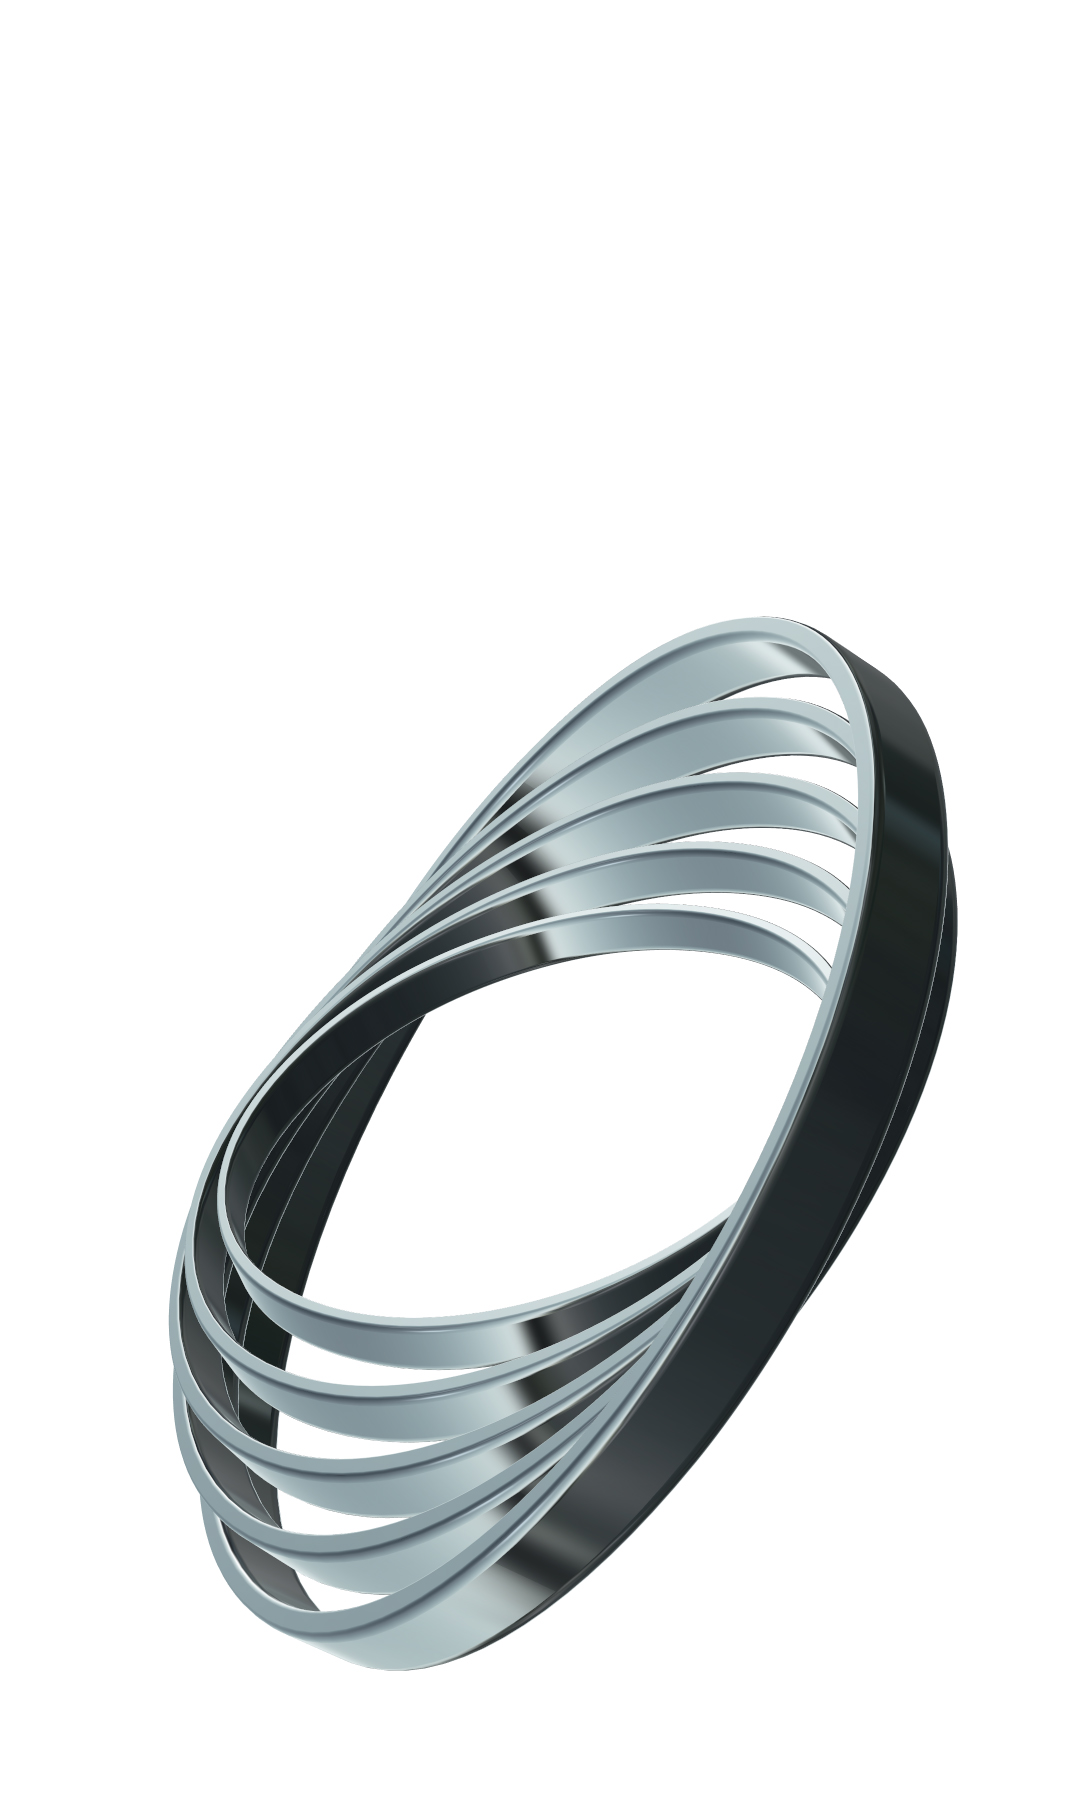
\includegraphics[trim={0 0 0 17cm},width=\paperwidth,height=\paperheight]{pictures/BG5.jpg}}
}
%----------------------------------------------------------------------------------------
%	NAME AND CONTACT INFORMATION SECTION
%----------------------------------------------------------------------------------------

\firstname{Antonius} % Your first name
\familyname{Torode} % Your last name

% All information in this block is optional, comment out any lines you don't need
\title{Curriculum vitae}
\address{7700 Austere drive}{Waterford, Michigan 48329}
\mobile{517-512-3580}
%\phone{None}
\email{AWTorode@gmail.com}
\homepage{msu.edu/~torodean/}{https://msu.edu/{\raise.17ex\hbox{$\scriptstyle\sim$}}torodean/} % The first argument is the url for the clickable link, the second argument is the url displayed in the template - this allows special characters to be displayed such as the tilde in this example
%\extrainfo{Contact via e-mail is best}
%\photo[70pt][0.4pt]{pictures/picture_me} % The first bracket is the picture height, the second is the thickness of the frame around the picture (0pt for no frame)
%\quote{}

%----------------------------------------------------------------------------------------

\begin{document}

\makecvtitle % Print the CV title

%----------------------------------------------------------------------------------------
%	EDUCATION SECTION
%----------------------------------------------------------------------------------------

\section{Education}

\cventry{2015--2018}{B.S., Physics, Mathematics (Duel Majors)}{Michigan State University}{East Lansing MI}{\textit{GPA -- 3.76}}{Finished all requirements for an undergraduate physics degree and Mathematics degree. Graduating at the end of Summer 2018.}
\cventry{2011--2014}{Undergraduate Studies}{Oakland Community College}{}{\textit{GPA -- 3.7}}{General studies as well as math/sciences up to and including Calculus III, Differential Equations, Engineering Physics II and General Chemistry II (4.0 in all).}
\cventry{2008--2011}{High School}{Clarkston High School}{Clarkston MI}{\textit{GPA -- 4.0 (ACT standards)}}{AP Physics, AP Calculus, AP Computer Sciences, CSMTech (3 year advanced math, science and technology program).}  % Arguments not required can be left empty

%----------------------------------------------------------------------------------------
%	WORK EXPERIENCE SECTION
%----------------------------------------------------------------------------------------

\section{Experience}

%\subsection{Vocational}

\cventry{2017--Present}{Undergraduate Research Assistant}{\textsc{National Superconducting Cyclotron Laboratory}}{East Lansing MI}{}{
\begin{itemize}
\item I work in experimental nuclear astrophysics.
\item My primary focus is with scintillator detectors and experimental setups to better understand nucleosynthesis.
\item  I also perform calculations and simulations for determining existing detector properties and new detector properties.
\end{itemize}}

%------------------------------------------------

\cventry{2016--Present}{P-A Computing Assistant}{\textsc{Michigan State University}}{East Lansing MI}{}{
\begin{itemize}
\item I work to manage and maintain the computers and networks for multiple departments at MSU, including Physics \& Astronomy, Phisiology, and Microbiology \& Molecular Genetics.
\item My responsibilities include fixing any common or difficult problems that may arise while applying my knowledge to maintain or improve efficiency within the department.
\end{itemize}}

%------------------------------------------------


\cventry{Summer 2016}{Physics Teaching Assistant}{\textsc{Michigan State University}}{East Lansing MI}{}{
\begin{itemize}
\item A weekly tutor and an exam proctor for PHY 232C, an online course taught at Michigan State University.
\item In charge of assisting students in the understanding of concepts and problems via both an online forum and in person.
\end{itemize}}
	
%------------------------------------------------


\cventry{2013--2015}{CRLA Certified Math, Physics and Chemistry Tutor}{\textsc{Oakland Community College}}{Auburn Hills MI}{}{
\begin{itemize}
\item Mathematics lab tutor for fundamental concepts and ideas including but not limited to mathematics, physics and chemistry.
\end{itemize}}

%------------------------------------------------

\cventry{Summer 2013}{Condensed Matter Physics Research}{\textsc{Oakland University}}{Auburn Hills MI}{}{
\begin{itemize}
\item Extensively studyied Raman spectroscopy and graphite/graphene under high pressures.
\item Performed a Raman spectroscopy experiment on graphene using a diamond anvil cell to achieve high pressures. 
\item Personally designed and set up resistivity experiments to confirm findings.
\item Presented research in a professional and comprehensive manner in front of an audience.
\end{itemize}}

%------------------------------------------------

\cventry{2011--2013}{Data Research Analyst}{\textsc{CLRS, inc.}}{Southfield MI}{}{
\begin{itemize}
\item Performed Data analysis of different financial markets including the General Motors commercial car market. 
\item Learned and filled in for other positions when needed, including management duties.
\item Performed analysis of economic markets and businesses.
\item In depth research of Las Vegas casino populations.
\item Analyzed business functionality and efficiency and improved upon them by shortening data verification process.
\end{itemize}}

%------------------------------------------------

\cventry{2010--Present}{d0sag3-Films}{\textsc{Home Business}}{}{}{
\begin{itemize}
\item d0sag3-Films is a video editing and graphic design title I created.
\item Paid projects for Detroit In Focus but also many personal projects. 
\item Many of my projects can be viewed at https://www.facebook.com/d0sag3 (d0sag3 is spelled with a zero).
\end{itemize}}

%----------------------------------------------------------------------------------------
%	PUBLICATIONS \& PROJECTS
%----------------------------------------------------------------------------------------

\section{Peer Reviewed Publications}

\cvitem{Jun 2017}{"Exploration of the Quantum Casimir Effect." Student Journal of Physics - International Version - Vol. 6. No. 2. April-June 2017 - Indian Association of Physics Teachers.}

\section{Other Publications and Projects}

\cvitem{2018}{"Multiple Integrated Applications (MIA)." Program created for further development of application design. Contains mathematical functions, encryption algorithms, windows key code simulations, a comprehensive workout generation system, and more.}
\cvitem{Oct 2017}{"Characterizing a Tape Station and Beta Detector For Radioactive Isotope Beam Experiments." Conference Poster presented at the Fall Meeting of the Division of Nuclear Physics of the American Physical Society}
\cvitem{2017}{"Generations of Nuclear Activity (GINA)." Program created for performing nuclear decay calculations for a new radioactive transport system at the NSCL.}
\cvitem{2017}{"Local Operations Listing Agent (LOLA)." Program created for improved efficiency and computer database management at MSU.}
\cvitem{May 2017}{"The Antonius Cookbook." Self Published: Free culinary cookbook download. https://msu.edu/{\raise.17ex\hbox{$\scriptstyle\sim$}}torodean/ACookbook.html}
\cvitem{Nov 2016}{"Antonius' Handbook." Comprehensive reference of useful formulas, constants, units and definitions. Self Published: Free book download for current version.
https://msu.edu/{\raise.17ex\hbox{$\scriptstyle\sim$}}torodean/AHandbook.html}

\newpage

%----------------------------------------------------------------------------------------
%	COMPUTER SKILLS SECTION
%----------------------------------------------------------------------------------------

\section{Computer skills}

\cvitem{Basic}{\textsc{php}, \textsc{Mac OS}}
\cvitem{Intermediate to Advanced}{Linux, \textsc{java}, \textsc{git}, \textsc{bash} \textsc{html}, \textsc{css}, \textsc{CAD}, \LaTeX, \textsc{C++}, \textsc{C\#}, Python, DS9, Stellarium, OpenOffice products, Microsoft Office products, Microsoft Windows 2000/XP/Vista/7/8/10, Adobe Premiere Pro, Adobe Illustrator, Sony Vegas, Final Cut Studio, Adobe Photoshop, Adobe After Effects, Cygwin Terminal, Qt, GNU/GCC compilation, makefile programming, Computer Hardware and Support, LabVIEW}



%----------------------------------------------------------------------------------------
%	AWARDS SECTION
%----------------------------------------------------------------------------------------

\section{Honors, Clubs, and Other Affiliations}

\cvitem{2016-2018}{Michigan State University Dean's List}
\cvitem{2017}{Lawrence W. Hantel Endowed Fellowship Fund, in Memory of Professor Donald J. Montgomery}
\cvitem{2016-2017}{Regular Attendee of Physics, Astronomy, and Karate Clubs at Michigan State University}
\cvitem{2015}{Member of the Phi Theta Kappa Honor Society}
\cvitem{2011-2015}{Oakland Community College Dean's List}
\cvitem{2010}{Member of the National Junior Classical League}

%----------------------------------------------------------------------------------------
%	COMMUNICATION SKILLS SECTION
%----------------------------------------------------------------------------------------

%\section{Communication Skills}

%\cvitem{2011--2012}{Composition I/II classes with various presentations}
%\cvitem{2013}{REU Condensed Matter Research presentation}

%----------------------------------------------------------------------------------------
%	LANGUAGES SECTION
%----------------------------------------------------------------------------------------

%\section{Languages}

%\cvitemwithcomment{English}{Mothertongue}{}
%\cvitemwithcomment{German}{Basic}{Basic words and phrases only}
%\cvitemwithcomment{Japanese}{Basic}{Basic words and phrases only}

%----------------------------------------------------------------------------------------
%	INTERESTS SECTION
%----------------------------------------------------------------------------------------

%\section{Interests and Hobbies}
%\cvitem{}{Mathematics, Chess, Chemistry,
%	Physics, Mathematics, Video Design, Computer Sciences, Health and Education, Technology}

%----------------------------------------------------------------------------------------
%	REFERENCES SECTION
%----------------------------------------------------------------------------------------

\section{References}

\cventry{2015--Present}{Artemis Spyrou}{Associate Professor of Physics, National Superconducting Cyclotron Laboratory}{Cyclotron, 640 S Shaw Ln, East Lansing, MI 48824}{spyrou@nscl.msu.edu (517)-908-7141}{Supervisor at NSCL.}
\cventry{2015--Present}{Esther V. V. Reed}{MSU Information Technologist
Departmental Support}{Biomed/Physical Science Building: 567 Wilson Road, Room 1209, East Lansing, MI 48824}{reed@pa.msu.edu (517)-884-5469}{Supervisor at Michigan State University.}
\cventry{2013--2015}{Michael Robinson}{OCC Faculty}{739 S Washington Ave, Royal Oak, MI 48067}{mdrobins@oaklandcc.edu (248)-232-4438}{Employer at Oakland Community College.}
\cventry{2011--2013}{Mitch Kanaan}{CLRS, inc. President/Owner}{29433 Southfield Road, Suite 106 Southfield, Michigan 48076}{mkanaan@clrsinc.com (248)-760-5316}{Employer at CLRS, Inc.}

%----------------------------------------------------------------------------------------
%	COVER LETTER
%----------------------------------------------------------------------------------------

% To remove the cover letter, comment out this entire block

%\clearpage

%\recipient{HR Department}{Corporation\\123 Pleasant Lane\\12345 City, State} % Letter recipient
%\date{\today} % Letter date
%\opening{Dear Sir or Madam,} % Opening greeting
%\closing{Sincerely yours,} % Closing phrase
%\enclosure[Attached]{curriculum vit\ae{}} % List of enclosed documents

%\makelettertitle % Print letter title

%\lipsum[1-3] % Dummy text

%\makeletterclosing % Print letter signature

%----------------------------------------------------------------------------------------

\end{document}